% Created by tikzDevice version 0.6.2-92-0ad2792 on 2012-09-15 22:55:20
% !TEX encoding = UTF-8 Unicode
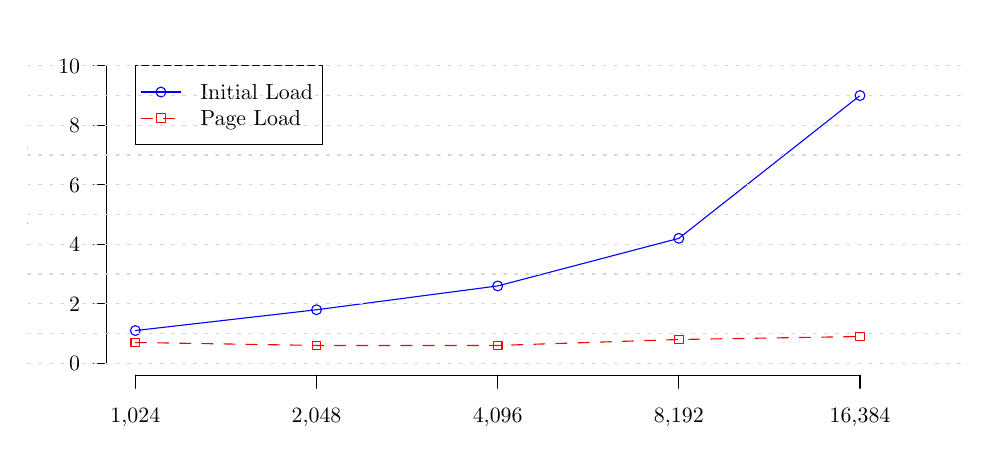
\begin{tikzpicture}[x=1pt,y=1pt]
\definecolor[named]{fillColor}{rgb}{1.00,1.00,1.00}
\path[use as bounding box,fill=fillColor,fill opacity=0.00] (0,0) rectangle (339.67,144.54);
\begin{scope}
\path[clip] (  0.00,  0.00) rectangle (339.67,144.54);
\definecolor[named]{drawColor}{rgb}{0.00,0.00,1.00}

\path[draw=drawColor,line width= 0.4pt,line join=round,line cap=round] ( 38.91, 35.09) --
	(104.37, 42.61) --
	(169.83, 51.21) --
	(235.29, 68.41) --
	(300.76,120.01);

\path[draw=drawColor,line width= 0.4pt,line join=round,line cap=round] ( 38.91, 35.09) circle (  1.78);

\path[draw=drawColor,line width= 0.4pt,line join=round,line cap=round] (104.37, 42.61) circle (  1.78);

\path[draw=drawColor,line width= 0.4pt,line join=round,line cap=round] (169.83, 51.21) circle (  1.78);

\path[draw=drawColor,line width= 0.4pt,line join=round,line cap=round] (235.29, 68.41) circle (  1.78);

\path[draw=drawColor,line width= 0.4pt,line join=round,line cap=round] (300.76,120.01) circle (  1.78);
\end{scope}
\begin{scope}
\path[clip] (  0.00,  0.00) rectangle (339.67,144.54);
\definecolor[named]{drawColor}{rgb}{0.00,0.00,0.00}

\path[draw=drawColor,line width= 0.4pt,line join=round,line cap=round] ( 38.91, 18.96) -- (300.76, 18.96);

\path[draw=drawColor,line width= 0.4pt,line join=round,line cap=round] ( 38.91, 18.96) -- ( 38.91, 14.22);

\path[draw=drawColor,line width= 0.4pt,line join=round,line cap=round] (104.37, 18.96) -- (104.37, 14.22);

\path[draw=drawColor,line width= 0.4pt,line join=round,line cap=round] (169.83, 18.96) -- (169.83, 14.22);

\path[draw=drawColor,line width= 0.4pt,line join=round,line cap=round] (235.29, 18.96) -- (235.29, 14.22);

\path[draw=drawColor,line width= 0.4pt,line join=round,line cap=round] (300.76, 18.96) -- (300.76, 14.22);

\node[text=drawColor,anchor=base,inner sep=0pt, outer sep=0pt, scale=  0.79] at ( 38.91,  1.90) {1,024};

\node[text=drawColor,anchor=base,inner sep=0pt, outer sep=0pt, scale=  0.79] at (104.37,  1.90) {2,048};

\node[text=drawColor,anchor=base,inner sep=0pt, outer sep=0pt, scale=  0.79] at (169.83,  1.90) {4,096};

\node[text=drawColor,anchor=base,inner sep=0pt, outer sep=0pt, scale=  0.79] at (235.29,  1.90) {8,192};

\node[text=drawColor,anchor=base,inner sep=0pt, outer sep=0pt, scale=  0.79] at (300.76,  1.90) {16,384};

\path[draw=drawColor,line width= 0.4pt,line join=round,line cap=round] ( 28.44, 23.26) -- ( 28.44,130.76);

\path[draw=drawColor,line width= 0.4pt,line join=round,line cap=round] ( 28.44, 23.26) -- ( 23.70, 23.26);

\path[draw=drawColor,line width= 0.4pt,line join=round,line cap=round] ( 28.44, 44.76) -- ( 23.70, 44.76);

\path[draw=drawColor,line width= 0.4pt,line join=round,line cap=round] ( 28.44, 66.26) -- ( 23.70, 66.26);

\path[draw=drawColor,line width= 0.4pt,line join=round,line cap=round] ( 28.44, 87.76) -- ( 23.70, 87.76);

\path[draw=drawColor,line width= 0.4pt,line join=round,line cap=round] ( 28.44,109.26) -- ( 23.70,109.26);

\path[draw=drawColor,line width= 0.4pt,line join=round,line cap=round] ( 28.44,130.76) -- ( 23.70,130.76);

\node[text=drawColor,anchor=base east,inner sep=0pt, outer sep=0pt, scale=  0.79] at ( 18.96, 20.54) {0};

\node[text=drawColor,anchor=base east,inner sep=0pt, outer sep=0pt, scale=  0.79] at ( 18.96, 42.04) {2};

\node[text=drawColor,anchor=base east,inner sep=0pt, outer sep=0pt, scale=  0.79] at ( 18.96, 63.54) {4};

\node[text=drawColor,anchor=base east,inner sep=0pt, outer sep=0pt, scale=  0.79] at ( 18.96, 85.04) {6};

\node[text=drawColor,anchor=base east,inner sep=0pt, outer sep=0pt, scale=  0.79] at ( 18.96,106.54) {8};

\node[text=drawColor,anchor=base east,inner sep=0pt, outer sep=0pt, scale=  0.79] at ( 18.96,128.04) {10};
\end{scope}
\begin{scope}
\path[clip] (  0.00,  0.00) rectangle (339.67,144.54);
\definecolor[named]{drawColor}{rgb}{1.00,0.00,0.00}

\path[draw=drawColor,line width= 0.4pt,dash pattern=on 4pt off 4pt ,line join=round,line cap=round] ( 38.91, 30.79) --
	(104.37, 29.71) --
	(169.83, 29.71) --
	(235.29, 31.86) --
	(300.76, 32.94);

\path[draw=drawColor,line width= 0.4pt,line join=round,line cap=round] ( 37.34, 29.21) rectangle ( 40.49, 32.36);

\path[draw=drawColor,line width= 0.4pt,line join=round,line cap=round] (102.80, 28.13) rectangle (105.95, 31.29);

\path[draw=drawColor,line width= 0.4pt,line join=round,line cap=round] (168.26, 28.13) rectangle (171.41, 31.29);

\path[draw=drawColor,line width= 0.4pt,line join=round,line cap=round] (233.72, 30.28) rectangle (236.87, 33.44);

\path[draw=drawColor,line width= 0.4pt,line join=round,line cap=round] (299.18, 31.36) rectangle (302.33, 34.51);
\definecolor[named]{drawColor}{rgb}{0.00,0.00,0.00}

\node[text=drawColor,rotate= 90.00,anchor=base,inner sep=0pt, outer sep=0pt, scale=  0.79] at ( -1.90, 77.01) {Time (seconds)};

\path[draw=drawColor,line width= 0.4pt,line join=round,line cap=round] ( 38.91,130.76) rectangle (106.63,102.32);
\definecolor[named]{drawColor}{rgb}{0.00,0.00,1.00}

\path[draw=drawColor,line width= 0.4pt,line join=round,line cap=round] ( 41.05,121.28) -- ( 55.27,121.28);
\definecolor[named]{drawColor}{rgb}{1.00,0.00,0.00}

\path[draw=drawColor,line width= 0.4pt,dash pattern=on 4pt off 4pt ,line join=round,line cap=round] ( 41.05,111.80) -- ( 55.27,111.80);
\definecolor[named]{drawColor}{rgb}{0.00,0.00,1.00}

\path[draw=drawColor,line width= 0.4pt,line join=round,line cap=round] ( 48.16,121.28) circle (  1.78);
\definecolor[named]{drawColor}{rgb}{1.00,0.00,0.00}

\path[draw=drawColor,line width= 0.4pt,line join=round,line cap=round] ( 46.58,110.22) rectangle ( 49.73,113.38);
\definecolor[named]{drawColor}{rgb}{0.00,0.00,0.00}

\node[text=drawColor,anchor=base west,inner sep=0pt, outer sep=0pt, scale=  0.79] at ( 62.38,118.56) {Initial Load};

\node[text=drawColor,anchor=base west,inner sep=0pt, outer sep=0pt, scale=  0.79] at ( 62.38,109.08) {Page Load};
\definecolor[named]{drawColor}{rgb}{0.83,0.83,0.83}

\path[draw=drawColor,line width= 0.4pt,dash pattern=on 1pt off 3pt ,line join=round,line cap=round] (  0.00, 23.26) -- (339.67, 23.26);

\path[draw=drawColor,line width= 0.4pt,dash pattern=on 1pt off 3pt ,line join=round,line cap=round] (  0.00, 34.01) -- (339.67, 34.01);

\path[draw=drawColor,line width= 0.4pt,dash pattern=on 1pt off 3pt ,line join=round,line cap=round] (  0.00, 44.76) -- (339.67, 44.76);

\path[draw=drawColor,line width= 0.4pt,dash pattern=on 1pt off 3pt ,line join=round,line cap=round] (  0.00, 55.51) -- (339.67, 55.51);

\path[draw=drawColor,line width= 0.4pt,dash pattern=on 1pt off 3pt ,line join=round,line cap=round] (  0.00, 66.26) -- (339.67, 66.26);

\path[draw=drawColor,line width= 0.4pt,dash pattern=on 1pt off 3pt ,line join=round,line cap=round] (  0.00, 77.01) -- (339.67, 77.01);

\path[draw=drawColor,line width= 0.4pt,dash pattern=on 1pt off 3pt ,line join=round,line cap=round] (  0.00, 87.76) -- (339.67, 87.76);

\path[draw=drawColor,line width= 0.4pt,dash pattern=on 1pt off 3pt ,line join=round,line cap=round] (  0.00, 98.51) -- (339.67, 98.51);

\path[draw=drawColor,line width= 0.4pt,dash pattern=on 1pt off 3pt ,line join=round,line cap=round] (  0.00,109.26) -- (339.67,109.26);

\path[draw=drawColor,line width= 0.4pt,dash pattern=on 1pt off 3pt ,line join=round,line cap=round] (  0.00,120.01) -- (339.67,120.01);

\path[draw=drawColor,line width= 0.4pt,dash pattern=on 1pt off 3pt ,line join=round,line cap=round] (  0.00,130.76) -- (339.67,130.76);
\end{scope}
\end{tikzpicture}
